\section{Application: military alliances 1816--2018}\label{sec:application}

\subsection{Data and model}
The Alliance Treaty Obligations and Provisions project \citep{leeds2002} records for every pair of states and year whether an alliance with a defense pledge was in effect; we use version 5.1 as distributed with the R package \texttt{peacesciencer} \citep{miller2022}, together with the Correlates of War list of state system members (version 2016).
Every maximal run of consecutive years in which a pair has a defense pledge becomes one interval of a symmetric link \ttt{defense}, established at the start of its first year and terminated at the start of the year after its last one.
Membership of a state in the international system is a link \ttt{[state, is in, system]} to a single hub entity.
This gives \AtopStates\ states, \AtopIntervals\ pact intervals (\AtopCensored\ still in effect in 2018) and \AtopEvents\ events (Fig.~\ref{fig:atop}, left).
The model has six metaparameters:
\par\noindent\begin{minipage}{\linewidth}
\begin{lstlisting}[language=yaml]
[state, defense, state]:
  establish:
    attempt:
      [~, is in, system, contains, ~]: a0  # per direction
      [~, defense, state, defense, ~]: a1  # per ally
    success: inf
  terminate:
    attempt:
      base: d0
    success:
      tails: 0
      [~, defense, state, defense, ~]: -b1 # per ally
[state, is in, system]: rates "entry", "exit"
\end{lstlisting}
\end{minipage}
\noindent Formation thus needs both states to be members (the angle through the hub), and its rate
grows linearly in the number of common allies; dissolution attempts succeed with probability $\expit(-4 b_1 k)$ for $k$ common allies.
Since \ttt{defense} is symmetric, both directed links of a pair are possible events with these rates, so a pair of member states forms a pact at the rate $2(a_0 + a_1 k)$ and a pact dissolves at the hazard $2 d_0 \expit(-4 b_1 k)$ (Sec.~\ref{sec:model}).

Two features of the data need a convention.
Pledges are recorded per year, so events of the same year are simultaneous; we order them as terminations, exits, entries, formations, and formations by state codes.
And a multilateral treaty appears as many dyadic events in one year, so that the later ones already see the earlier ones as common allies.
With a random order of the events within a year, the estimates change by the amounts discussed below.

\subsection{Results}
Table~\ref{tab:atop} reports the maximum-likelihood estimates.
A pair of member states without a common ally forms a pact at a rate of $2a_0 = \AtopPairAzero$ per year; each common ally adds $2a_1 = \AtopPairAone$, so that one common ally raises the formation rate about \AtopFormationRatio-fold.
The dissolution hazard is $2 d_0\,\expit(-4 b_1 k)$: \AtopHazZero\ per year without common allies (a mean pact duration of \AtopLifeZero\ years), \AtopHazFive\ with five and \AtopHazTwentySix\ with 26, the size of NATO in 2004 (Fig.~\ref{fig:atop}, right).
Both effects are strongly supported: removing the ally-of-ally term from the formation rule lowers the maximal log-likelihood by \AtopDropAone, removing the stabilization term by \AtopDropBone.
With a random order of the simultaneous events, $a_0$ changes by \AtopShuffleAzero\%, $a_1$ by \AtopShuffleAone\% and $b_1$ by \AtopShuffleBone\%, so the formation effect partly reflects treaty-level events, which a model with an explicit treaty entity type could separate.

The profile log-likelihood of $b_1$ (Fig.~\ref{fig:atop}, middle) is not unimodal. Below a local minimum at small negative values it rises again towards a plateau as $b_1 \to -\infty$, where any common ally makes every dissolution attempt succeed; the plateau lies about \AtopProfileGap\ log-likelihood units below the maximum.
An optimizer started at negative values drifts towards the plateau, which illustrates the non-concavity in the probability units noted in Sec.~\ref{sec:inference}; the generated model therefore starts the fit at a positive value.
A likelihood evaluation of the \AtopEvents\ events takes about \AtopEvalSeconds\ seconds, a complete fit with standard errors about a minute.

\begin{table*}[t]
\caption{Maximum-likelihood estimates for the alliance model (standard errors from the observed information).
Rates per year.}
\label{tab:atop}
\begin{tabular}{llrr}
\toprule
parameter & meaning & estimate & s.e. \\
\midrule
$a_0$ & formation rate per pair of member states & $1.78\times 10^{-4}$ & $8.2\times 10^{-6}$ \\
$a_1$ & additional formation rate per common ally & $0.0102$ & $2.0\times 10^{-4}$ \\
$d_0$ & dissolution attempt rate & $0.108$ & $0.0048$ \\
$b_1$ & probability units per common ally (dissolution) & $0.0371$ & $9.2\times 10^{-4}$ \\
entry & entry rate of states & $0.00806$ & $5.4\times 10^{-4}$ \\
exit & exit rate of states & $0.00315$ & $4.4\times 10^{-4}$ \\
\midrule
\multicolumn{2}{l}{log-likelihood} & \multicolumn{2}{r}{$-20\,841.2$} \\
\bottomrule
\end{tabular}

\end{table*}

\begin{figure*}[t]
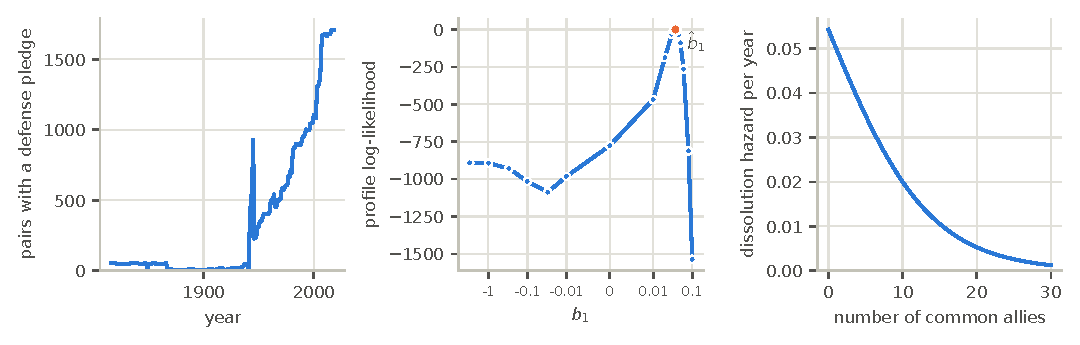
\includegraphics[width=\textwidth]{generated/fig-atop}
\caption{Defense pacts between states.
Left: number of pairs of states with a defense pledge in effect, per year.
Middle: profile log-likelihood of the stabilization parameter $b_1$ (all other parameters re-estimated), relative to its maximum (symmetric-log horizontal axis).
Right: estimated dissolution hazard as a function of the number of common allies.}
\label{fig:atop}
\end{figure*}
